\section{Graphendurchmusterung}
Graphen müssen häufig durchmustert, d.h systematisch durchsucht, werden. Im Folgenden werden wir die "Tiefensuche" und die "Breitensuche" betrachten, welche sich beide auf den folgenden Algorithmus zurückführen lassen:\\

\begin{algorithm}[H]
\label{alg:algorithmische_suche}
\caption{Algorithmische Suche}
\KwData{Graph $G=(V,E)$, Startknoten $s \in V$}
\KwResult{Zusammenhängender, azyklischer Graph $G'(R,T)$ mit $R=\{s\} \cup post^{*}(s)$ und $T \subset E$}
\begin{itemize}
	\item $R=\{s\}$
	\item $Q= \{s\}$
	\item $T= \emptyset$
	\item (a) \If{$Q= \emptyset$}{stop}
		\Else{Wähle $v \in  Q \subset R$}
	\item Wähle $w \in  V \setminus R \cap post(v)$
		\If{ kein solches $w$ exisitert}{setze $Q= Q \setminus \{v\}$ und gehe zu (a)}
	\item $R=R \cup \{w\}$
	\item $Q=Q \cup \{w\} $
	\item $T= T \cup \{e\} $ mit $e=(v,w)$ oder $e=\{v,w\} $
	\item Gehe zu (a)
\end{itemize}
\end{algorithm}
Je nachdem wie $v \in Q$ gewählt wird, bezeichnen wir den Suchalgorithmus unterschiedlich:
\begin{definition}
Bei der \emph{Tiefensuche} oder \emph{Depth-First-Search} (DFS) wird derjenige Knoten in $v \in  Q$ ausgewählt, der zuletzt zu $Q$ hinzugefügt wurde. Bei der \emph{Breitensuche} oder \emph{Breadth-First-Search} (BSF) wird derjenige Knoten $v \in  Q$ ausgewählt, der zuerst zu Q hinzugefügt wurde.
\end{definition}
\begin{theorem}
Algorithmus \ref{alg:algorithmische_suche} liefert einen zusammenhängenden, azyklischen Graphen $G'(R,T)$, mit $R=\{s\}\cup post^{*}(s)$ und $T \subset E$.
\end{theorem}
\begin{proof}
Per Konstruktion ist $(R,T)$ zu jedem Zeitpunkt im Algorithmus zusammenhängend.\\
$(R,T)$ ist außerdem zu jedem Zeitpunkt azyklisch, denn per Konstruktion gilt $Q \subset R$ und $e$ verbindet jeweils $v \in  Q \subset R$ mit $w \in  V \setminus R$. Wir müssen also zeigen: $R = \{s\} \cup post^{*}(v)$ ($T \subset E$ ist klar). \\
\underline{Annahme:} Nach Ende des Algorithmus gibt es $w \in  V \setminus R$ von $s$ erreichbar. Dann gibt es einen Weg \[
\pi = s,v_1,\ldots,v_r, w
\]
und darin eine Kante $e=(x,y) \in E$ bzw. $e >\{x,y\} \in E$, mit $x \in R$ und $y \not\in R$, $x,y \in \{s,v_1,\ldots,v_r,w\} $.
Da $x \in  R$, muss zu einem gewissen Zeitpunkt im Algorithmus auch $x \in  Q$ gelten. Der Algorithmus terminiert, aber nur, falls $x$ aus $Q$ entfernt wurde, was nur geschieht, wenn $y \not\in V \setminus R \cap post(x)$, also falls $e \not\in E$ ist. \\
Dies ist ein Widerspruch zu unserer Annahme.
\end{proof}
\begin{example}
Betrachte 
\begin{center}
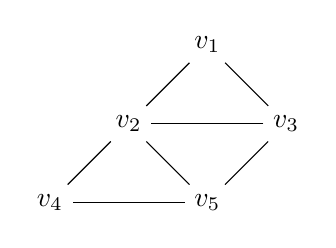
\begin{tikzpicture}
 \node (v1) at (0,0) {$v_1$};
 \node (v2) at (-1,-1) {$v_2$};
 \node (v3) at (1,-1) {$v_3$};
 \node (v4) at (-2,-2) {$v_4$};
 \node (v5) at (0,-2) {$v_5$};

 \path [-] (v1) edge node {} (v2);
 \path [-] (v1) edge node {} (v3);
 \path [-] (v3) edge node {} (v2);
 \path [-] (v4) edge node {} (v2);
 \path [-] (v5) edge node {} (v2);
 \path [-] (v5) edge node {} (v4);
 \path [-] (v3) edge node {} (v5);
\end{tikzpicture}
\end{center}
$s =\{v_1\}$. Bei der Tiefensuche entsteht folgender Baum:
\begin{center}
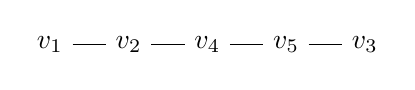
\begin{tikzpicture}
\node (v1) at (0,0) {$v_1$};
\node (v2) at (1,0) {$v_2$};
\node (v3) at (4,0) {$v_3$};
\node (v4) at (2,0) {$v_4$};
\node (v5) at (3,0) {$v_5$};

\path [-] (v1) edge node {} (v2);
\path [-] (v2) edge node {} (v4);
\path [-] (v4) edge node {} (v5);
\path [-] (v5) edge node {} (v3);
\end{tikzpicture}
\end{center}
Die Breitensuche hingegen ergibt:
\begin{center}
\begin{tikzpicture}
\node (v1) at (0,0) {$v_1$};
\node (v2) at (-1,-1) {$v_2$};
\node (v3) at (1,-1) {$v_3$};
\node (v4) at (-2,-2) {$v_4$};
\node (v5) at (0,-2) {$v_5$};

\path [-] (v1) edge node {} (v2);
\path [-] (v1) edge node {} (v3);
\path [-] (v2) edge node {} (v4);
\path [-] (v2) edge node {} (v5);	
\end{tikzpicture}
\end{center}
\end{example}
\begin{remark}
Ist $G$ ein ungerichteter Graph, so ist das Resultat $G'$ von Algorithmus \ref{alg:algorithmische_suche} ein Baum mit Wurzel $s$, der \emph{Spannbaum}
\end{remark}
\begin{theorem}
	\label{thm:algorithmische_suche}
	Die Ausführung von "wähle $v \in Q$" und "wähle $w \in  V \setminus R \cap post(v)$" sei in $\mathcal{O}(1)$ durchführbar. Dann besitzt Algorithmus \ref{alg:algorithmische_suche} den linearen Aufwand $\mathcal{O}(|V|+|E|)$.
\end{theorem}
\begin{proof}
"wähle $v \in Q$" wird maximal $(|post(v)|+1)$ mal aufgerufen. \\
"wähle $w \in V \setminus R \cap post(v)$" wird für jede Kante maximal ein mal aufgerufen. \\
Daraus folgt direkt die Behauptung.
\end{proof}
Wir hatten gezeigt, (Satz \ref{thm:zusammenhang}), dass $|V|-1 \le |E|$, d.h, es gilt $\mathcal{O}(|V|+|E|)$ kann nach oben beschränkt werden durch $\mathcal{O}(2|E|)$.
\paragraph{Beobachtung:} Die Breitensuche beschreibt einen "kürzesten" Weg von Startknoten zu jedem anderen Knoten.

\begin{theorem}
	Sie $G=(V,E)$ ein ungerichteter Graph, $s,v \in V$ und \\ $dist_G(s,v)= \min \{|\pi| : \pi = s,u_1,\ldots,u_r,v \text{ ein Weg in G}\}$ mit $dist_G(s,v) = \infty $, falls es keinen Weg von $s$ nach $v$ gibt. 
Dann enthält der durch die Breitensuche erzeugte Graph $G'=(R,T)$ zum Startknoten $s \in V$ einen kürzesten Weg zu jedem Knoten $v \in  post^{*}(s)$.Dies bedeutet, es gib einen einfachen Weg $\pi=s,u_1,\ldots,u_r,v$ in $G'$ mit $|\pi|= dist_{G'}(s,v)= dist_G(s,v)$ minimal.
\end{theorem}
\begin{proof}
Wir bemerken zuerst, dass $G'$ azyklisch ist und somit $\pi$ in $G'$ eindeutig bestimmt ist.
Modifiziere Algorithmus \ref{alg:algorithmische_suche} nun wie folgt:
\begin{itemize}
	\item In 1: l(s)=0
	\item In 4: l(w) = l(v)+1
\end{itemize}
Dies bedeutet, zu jedem Zeitpunkt im Algorithmus gilt:
\[
l(v)=dist_{(R,T)} (s,v) , v \in R
\]
Insbesondere gibt es für kein in 2 ausgewähltes $v \in  Q$ ein $w \in R$ mit:
\begin{equation}
	\label{eqn:dist1}
l(w)> l(v)+1
\end{equation}
\underline{Zu Zeigen:} $dist_{R,T} (s,v) = dist_{G'} (s,v) = dist_G (s,v)$ \\
\underline{Annahme:} Nach Abbruch des Algorithmus gibt es ein $w \in V$ mit 
\begin{equation}
\label{eqn:dist2}
dist_G(s,w) < dist_{G'} (s,w)
\end{equation}
Falls es mehr als ein solches $w$  gibt , wähle dasjenige mit den kleinsten Abstand 
$dist_G(s,w)$.\\
Sei $\pi=s,u_1,\ldots,u_r,v,w \implies dist_G(s,v) = dist_{G'} (s,v)$ , da sonst v ein Knoten mit kleineren Abstand wäre, der \eqref{eqn:dist2} erfüllt.
\begin{align*}
	\implies l(w) &= dist_{G'}(s,w) \\
		      &> dist_G(s,w) \\
		      &= dist_G (s,v) +1 \\
		      &= dist_{G'} (s,v)+1 \\
		      &=l(v) +1
\end{align*}
Dies ist ein Widerspruch zu \eqref{eqn:dist1}.
\end{proof}
\begin{remark}
Die Breitensuche berechnet also die Wege aller Knoten zur Wurzel in $\mathcal{O}(|V|+|E|)$ .
\end{remark}
